\begin{figure}[t]
\centering
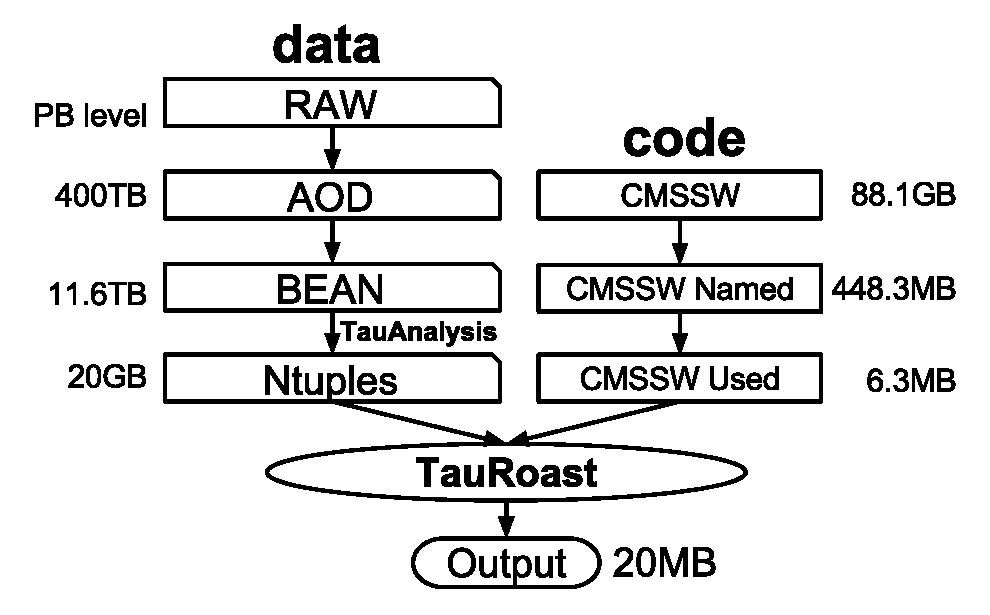
\includegraphics[width=.5\textwidth]{data-code-size.eps}
\caption{Inputs to Tau Roast}
\label{fig:data-code-size}
\end{figure}

\section{Overview of Tau Roast}

Within the ongoing investigation of the Higgs boson at the CMS
detector, part of the LHC at CERN~\cite{collaboration2008cms}, the Higgs production in association
with two top quarks allows measuring the Higgs coupling strength to
top quarks~\cite{chatrchyan2013search}.  As the Higgs boson is too short-lived to be detected
itself, it has to be reconstructed from its decay products.

The application which is the study of this paper is called \emph{TauRoast}.
It searches for cases where the Higgs boson decays to two tau leptons.
Since the tau leptons are very short-lived, they are not observed directly, but by the particle decay products 
that they generate.  So, the analysis must search for detector
events that show a signature of decay products compatible with both hadronic tau and top decays.  Properties of such events are used to distinguish
the events of interest (Higgs decays) from all other events and
are also used in further statistical analysis.

Figure~\ref{fig:data-code-size} shows that both the code and data
that form \emph{TauRoast} are drawn from large repositories through
multiple steps of reduction.  A preservation strategy must weigh
whether to store the large repositories completely, the fragments
used by an artifact, or something in between.

{\bf Code Sources.} Like many scientific codes, the central algorithm
of \emph{TauRoast} is expressed in a relatively small amount of
custom code developed by the primary author.  But, the code cannot
run at all without making use of an enormous collection of software
dependencies.  Some of these dependencies are standard to operating
systems worldwide, some are standardized across the entire high-energy
physics field, some are particular to small collaborative groups,
and a few are very specific to a single researcher.

The largest of these repositories is the CMS Software Distribution (CMSSW)~\cite{cms2006cms},
a carefully-curated selection of software packages which is distributed
in several forms.  Historically, components of CMSSW were obtained by checking components
of the source out of CVS (CMSSW source codes were moved from CVS to git recently), or by installing a complete binary package on a shared
filesystem within an HPC center.  In recent years, distribution has moved to
an on-demand delivery system known as CVMFS~\cite{blomer2011cernvm}, which
provides a filesystem interface that transparently accesses a remote repository.
The content of CMSSW is managed very carefully by a centralized team whose main goal
is to ensure that the current version of the software operates correctly
on the operating systems and architectures currently in use.  However,
preservation is not a specific objective of the system, and so there is
no particular guarantee that old versions of CMSSW will continue to
operate indefinitely.

CMSSW contains many different tools, libraries, and utilities.  No single code uses anywhere close to all of these.  But, because it is widely used within the experimental researchers, it is common for users to simply expect that a particular version of the entire repository is available.
 
{\bf Data Sources.}
The CMS collaboration provides end-users with a pre-processed
and reduced data format, AOD~\cite{holtman2001cms}, containing information for events, i.e.,
proton-proton collisions with a signature of interest, in the form of
reconstructed particles.  This format is based on the RAW output of
the CMS detector readout electronics and reconstructed world-wide, which is then processed through various algorithms which derive signatures of individual particles.
Both real and simulated data are available for examination.

As AOD data are too large to be iteratively processed repetitively in
a physics analysis workflow, it is normally reduced further in
structural complexity and content.  For the analysis under
investigation here, this is a two-step process.  First, the AOD data
are processed at the Notre Dame working group cluster to BEAN (Boson Exploration Analysis Ntuple) events,
containing only trivial data containers packed in vectors.  This step
is time and CPU intensive and its output contains data of 11.6$\,$TB to be
analyzed by the tau analysis.
It is performed by a small custom code framework, which is built on top of CMSSW.
The BEAN format, production code, and
data are shared within the analysis group looking at Higgs production
in association with top quarks, which is formed by groups from a few
American and European universities,
consisting of up to a few dozen contributors.

In the second step, the data are reduced to the ``Ntuple'' format,
which contains only events matching basic quality criteria and
fields relevant to \emph{TauRoast}.
Again, the Notre Dame CMS groups cluster
resources are used to perform this reduction and selection,
running highly customized software,
built on CMSSW and the BEAN framework,
with code written and maintained by a small group.

Once the data has been reduced to Ntuples, TauRoast can be run as a single
process, and contains a stringent event selection to look only at high
quality candidate events for the underlying physical process.
Quantities from the relevant events can be
both plotted and used in multivariate analysis to determine the level
of expected signal in real data.
This package is written using the CMSSW build framework,
but only utilizes code from ROOT,
a particle physics toolkit underlying CMSSW,
and a few external python dependencies for convenience.

